\begin{figure*}
    % \begin{minipage}[b]{0.63\linewidth}
        % \centering
    %    \hspace{-5mm}
    {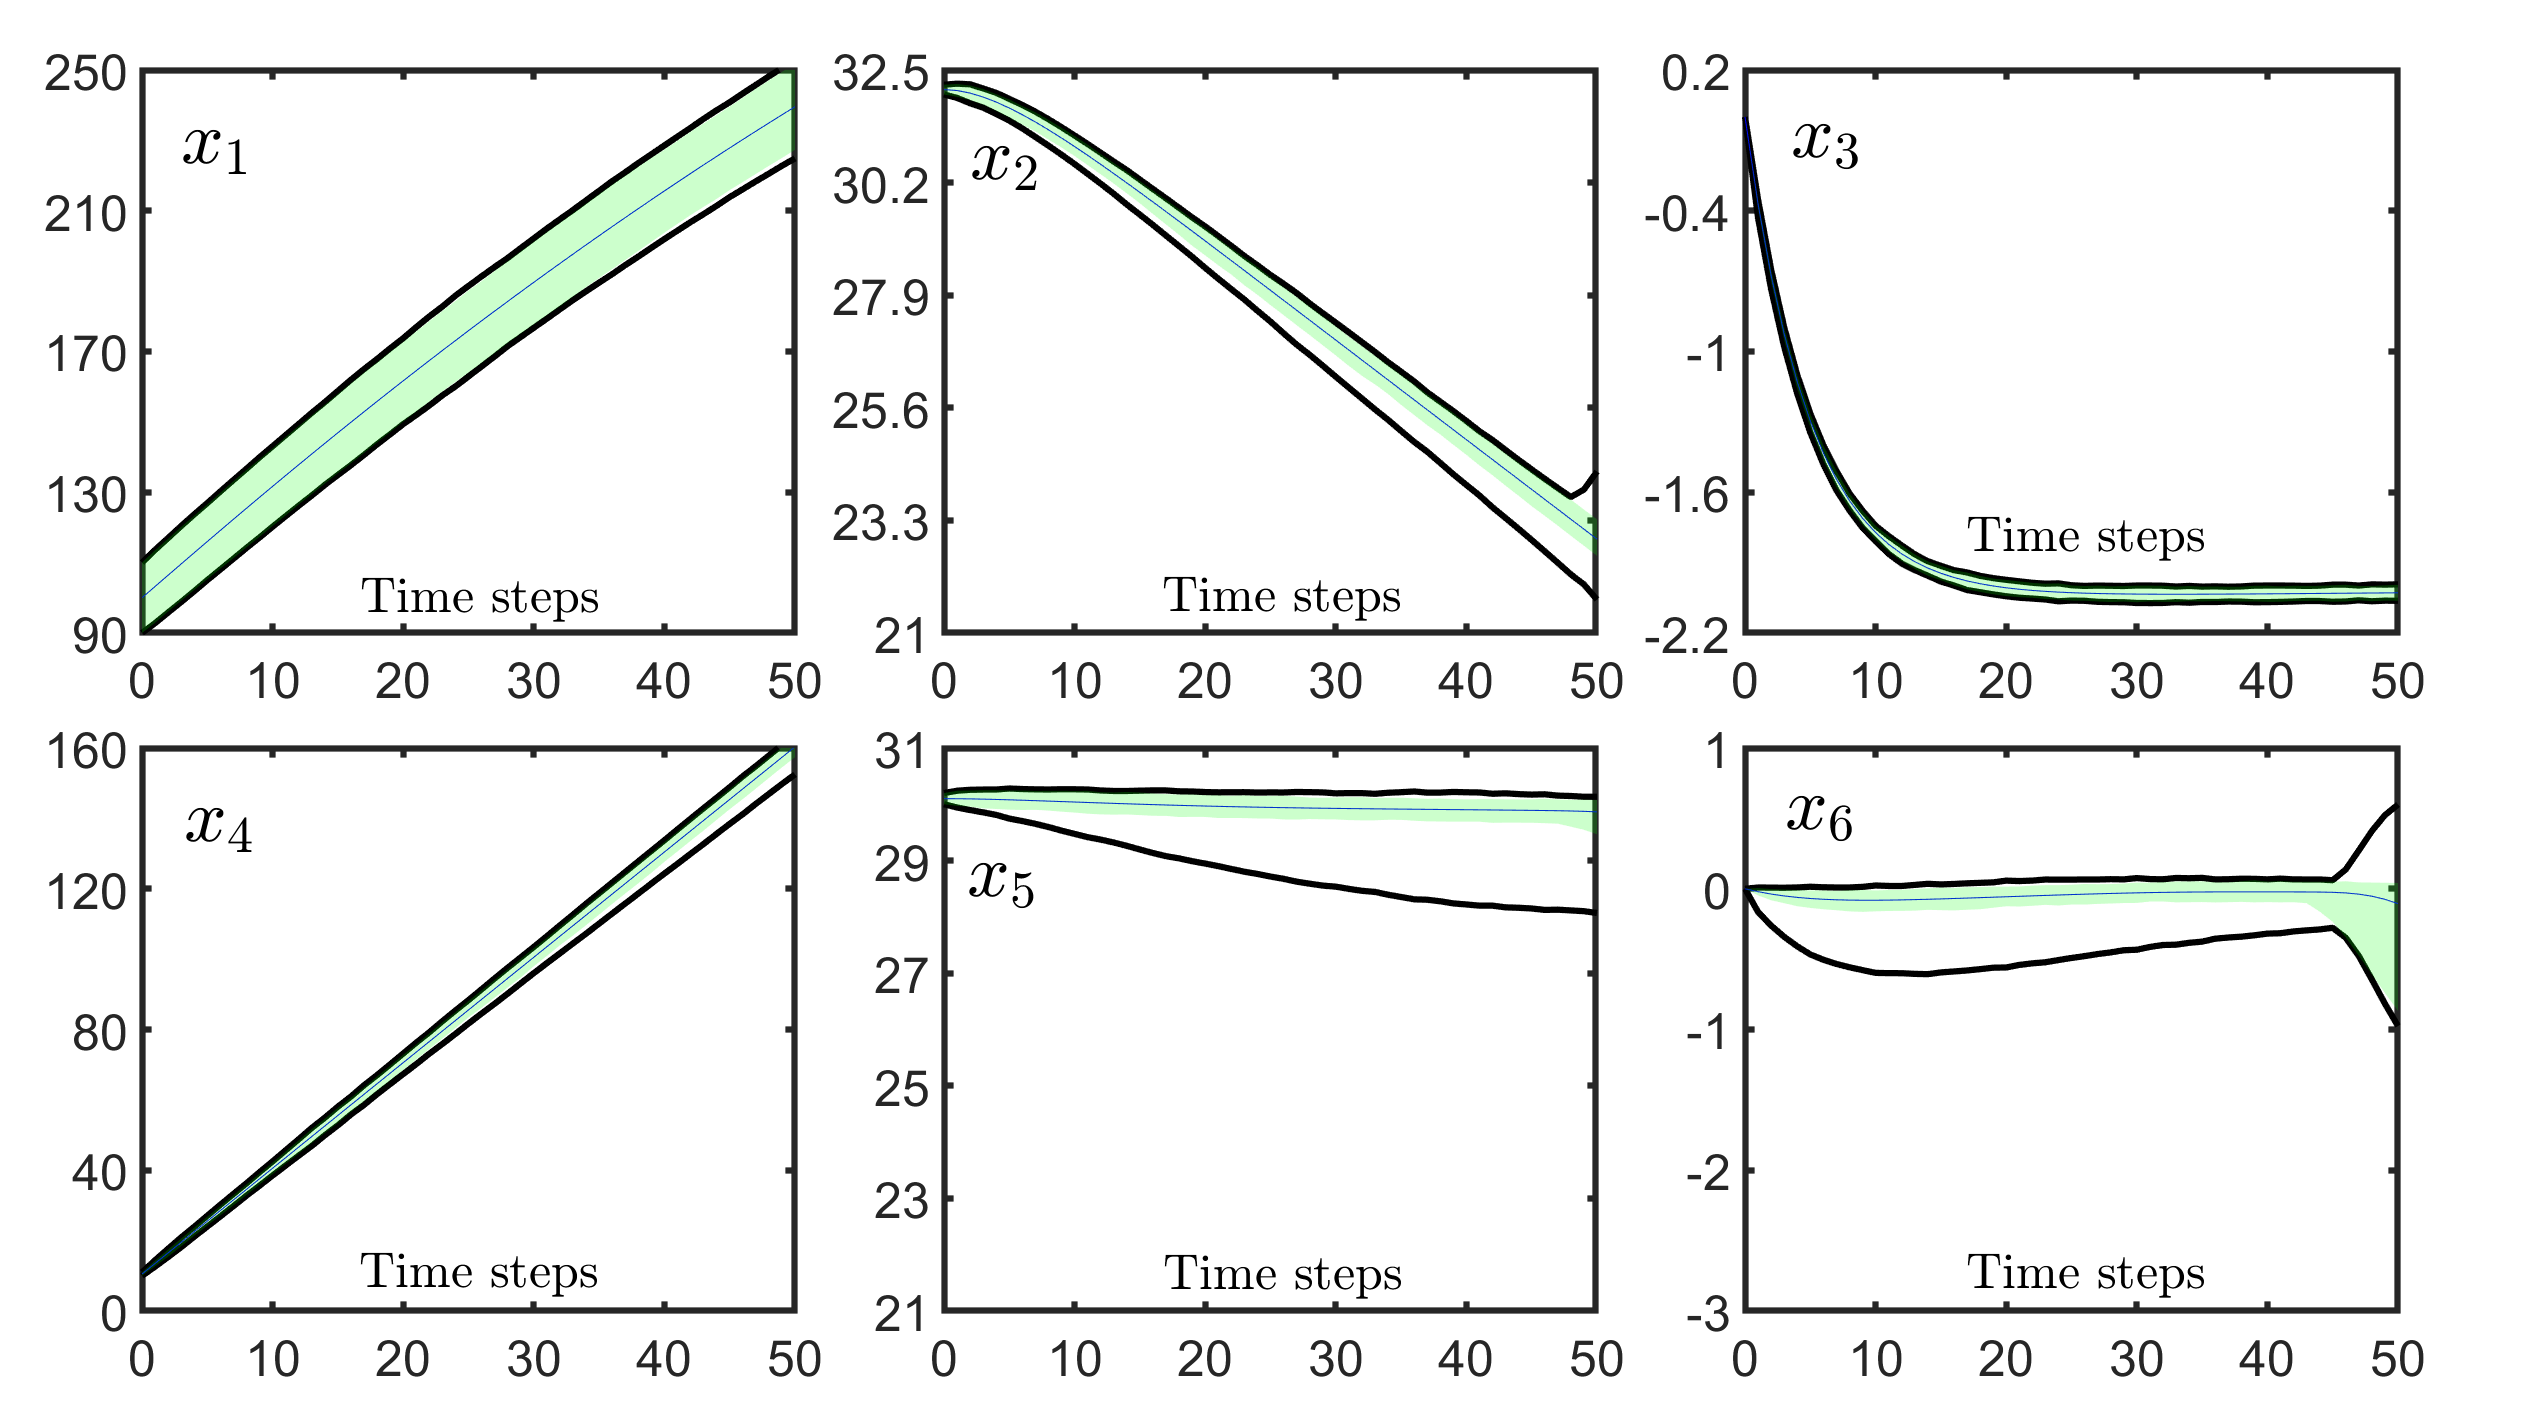
\includegraphics[width=1.0\linewidth]{figures/final_results_ACC.eps}}
    {\caption{Adaptive Cruise Control: The black lines indicate the probabilistic flowpipe computed using the exact-star technique on the learned surrogate model combined with conformal inference with failure probability $\varepsilon=0.01$. The green shaded areas and blue lines are computed from $100000$ random trajectories from the ODE model. The green area shows the maximum and minimum value of the trajectory components over this dataset, and the blue line represents their average value.}
    \label{fig:acc_comparison}}
    %\end{minipage}
    % \hfill 
    % \begin{minipage}[b]{0.35\linewidth} 
\end{figure*}

\begin{table}[t]
    \resizebox{\textwidth}{!}{
    \begin{tabular}{ccc||ccc} 
    \toprule
    Failure & Conformal inference & Reachability& Failure  & Conformal inference & Reachability  \\
     Probability & Run-time & Run-time & Probability & Run-time & Run-time \\ 
    \midrule \rowcolor{Gray}
    $0.10$ &   2.9439 $\mathrm{sec}$ & 9.8059 $\mathrm{sec}$ &  $0.05$ & 2.8783 $\mathrm{sec}$ &10.7457 $\mathrm{sec}$  \\
    $0.09$ &  2.8511 $\mathrm{sec}$ &9.0679 $\mathrm{sec}$  &  $0.04$ & 2.7901 $\mathrm{sec}$ &10.0033 $\mathrm{sec}$  \\
    \rowcolor{Gray}
    $0.08$ &  2.7367 $\mathrm{sec}$ &10.0502 $\mathrm{sec}$  &  $0.03$ & 3.096 $\mathrm{sec}$ &9.4364 $\mathrm{sec}$  \\
    $0.07$ &  2.8785 $\mathrm{sec}$ &9.7935 $\mathrm{sec}$ &  $0.02$ & 3.3982 $\mathrm{sec}$ &10.0027 $\mathrm{sec}$  \\
    \rowcolor{Gray}
    $0.06$ &  2.9341 $\mathrm{sec}$ &9.7988 $\mathrm{sec}$  & $0.01$ & 2.8536 $\mathrm{sec}$ &9.7945 $\mathrm{sec}$  \\
    \bottomrule
    \end{tabular}
    }
    \caption{Adaptive Cruise Control: Computation times of our method for different user-provided failure probabilities $\varepsilon$. The reachability run-time is the overall time for reachability analysis over the surrogate model and constructing the probabilistic flowpipe with conformal inference. The run-time for training a surrogate $\relu$ model was 2 hours and the run-time for test data-generation was 122 seconds.}  \label{tbl:acc}
\end{table}


% \begin{figure*}[t]
%     \centering
%     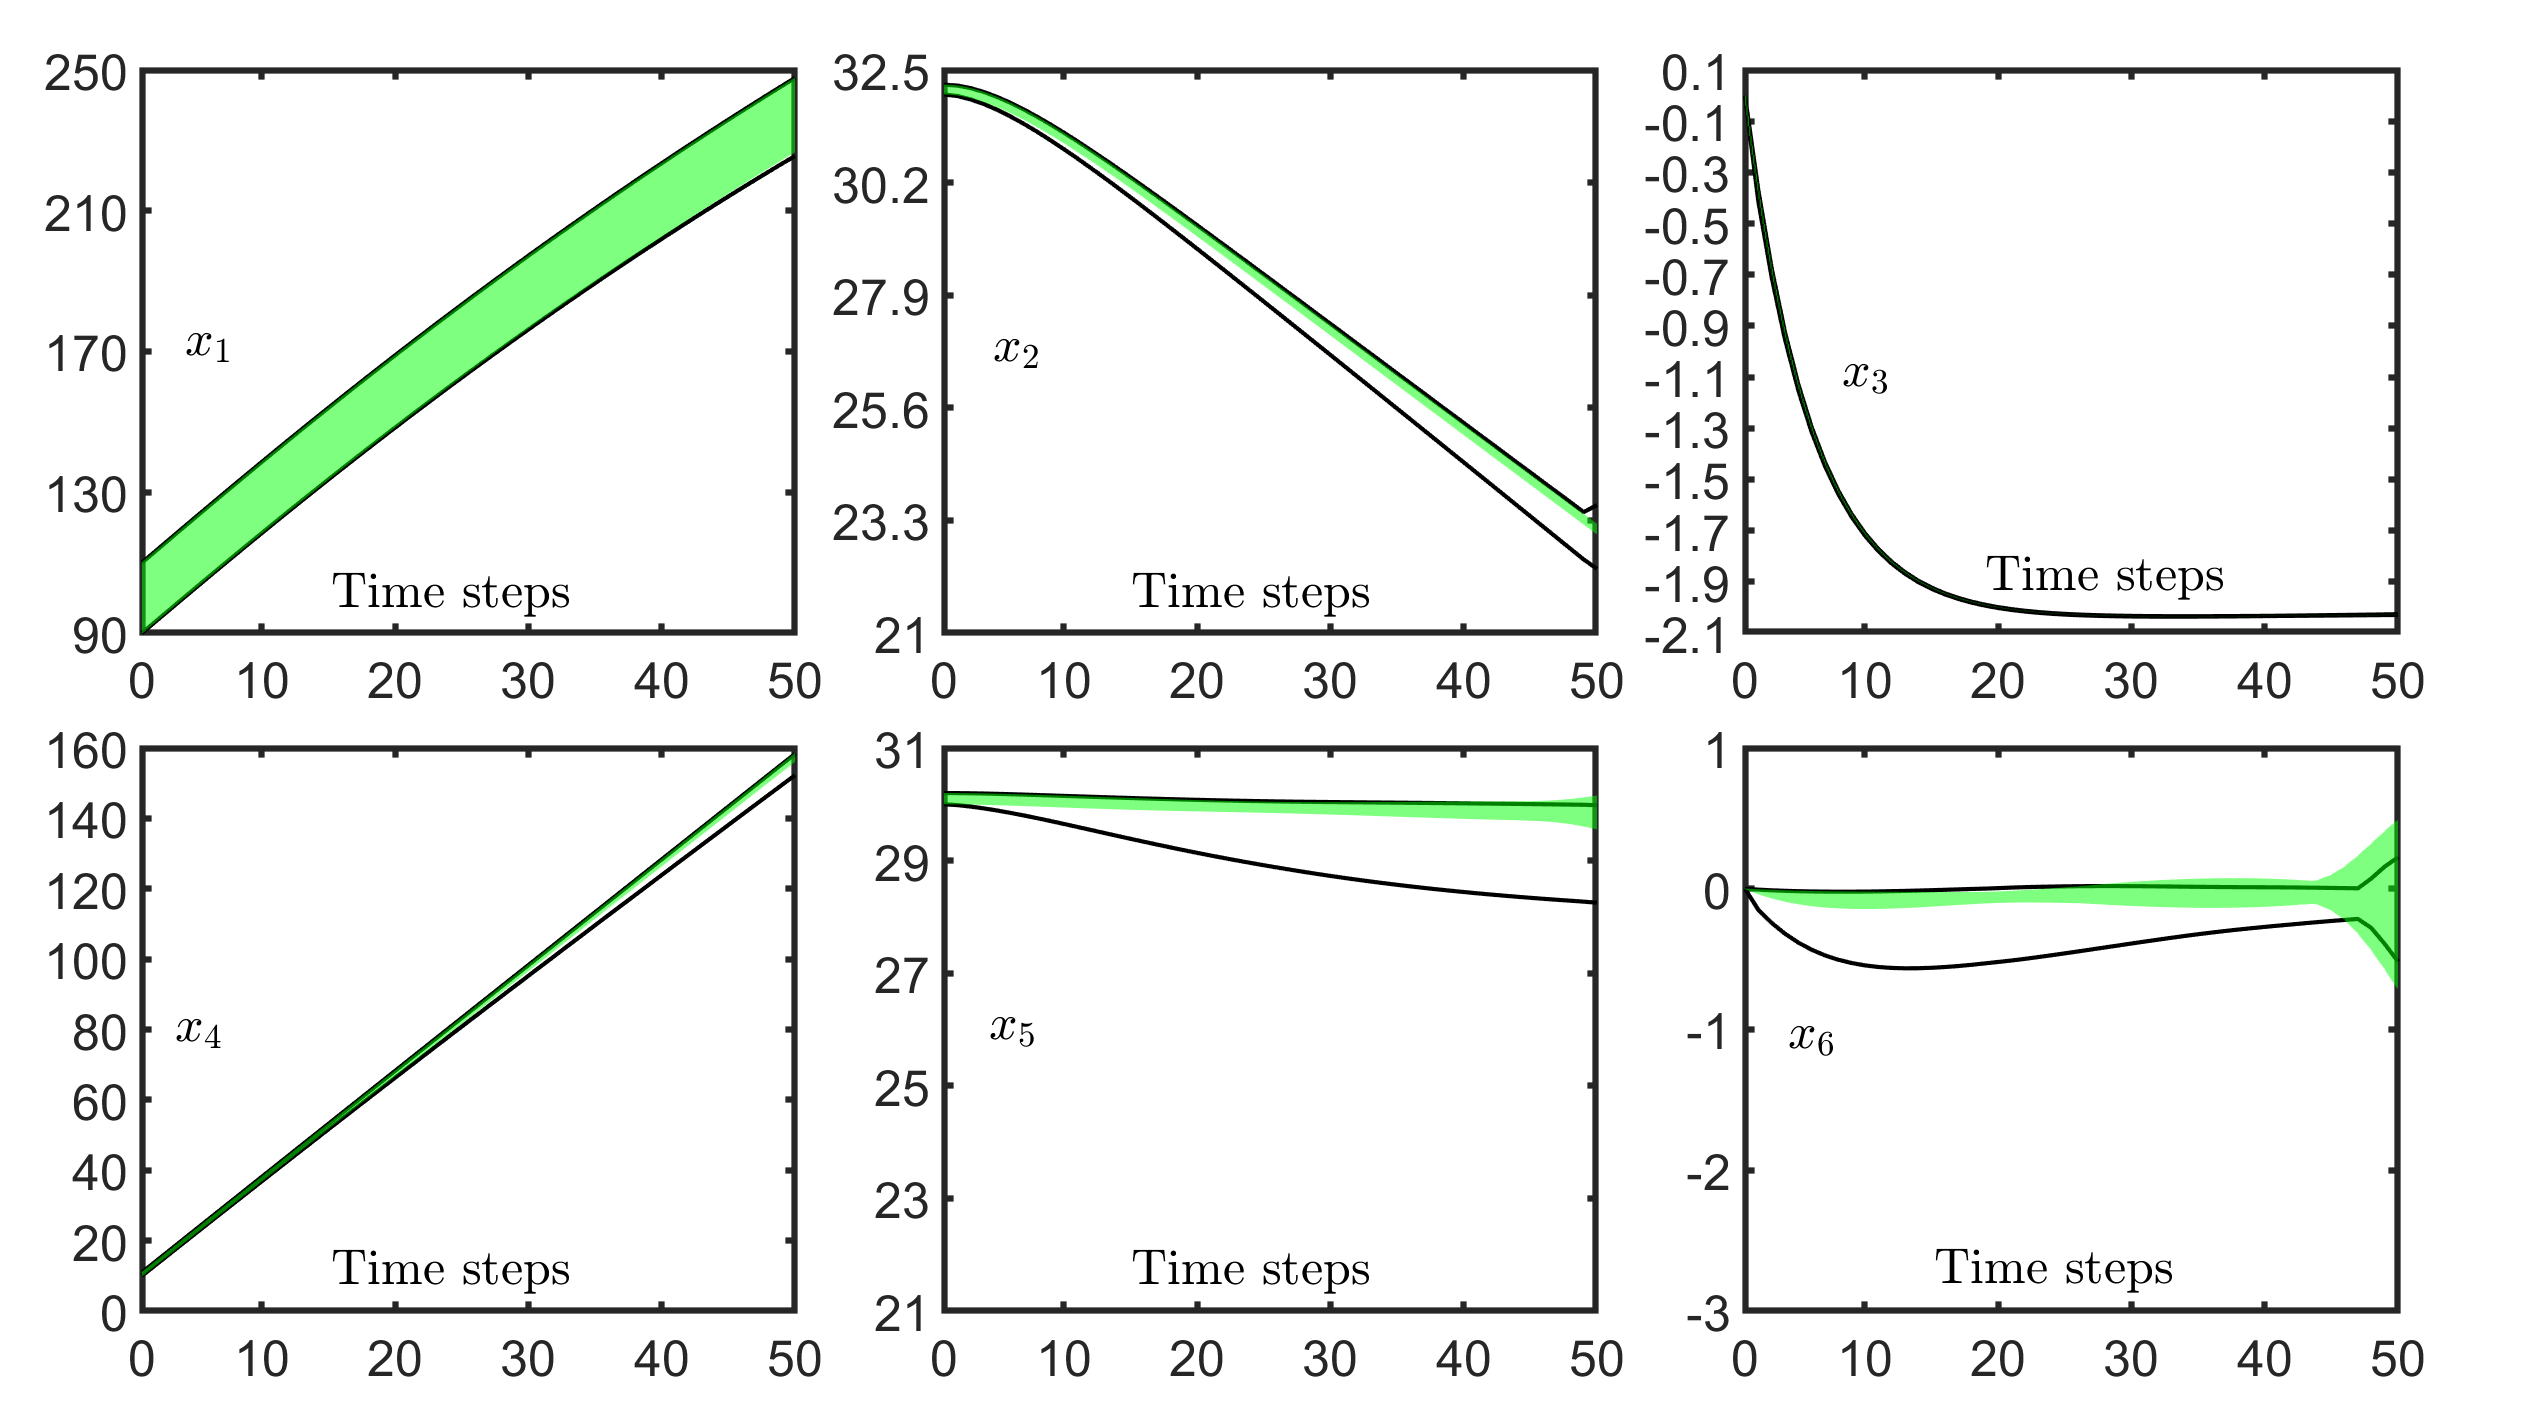
\includegraphics[width = 0.65\linewidth]{figures/Main_results.eps}
%     \caption{\small{Shows the  reachability analysis from $\horizon$-step dataset along with reachability analysis when the black-box model is ideally known. The bounds in black line shows the reachability analysis with exact-star technique combined with conformal inference with prescribed failure probability $\varepsilon=0.001$. The green reachset is derived from CORA \cite{althoff2015introduction} library and represent the tight upper bound for the black-box model in equation \eqref{eq:acc}, when the model is ideally known.}}
%     \label{fig:acc_comparison}
% \end{figure*}
\begin{figure*}[t]
    \hspace{-8mm}
    {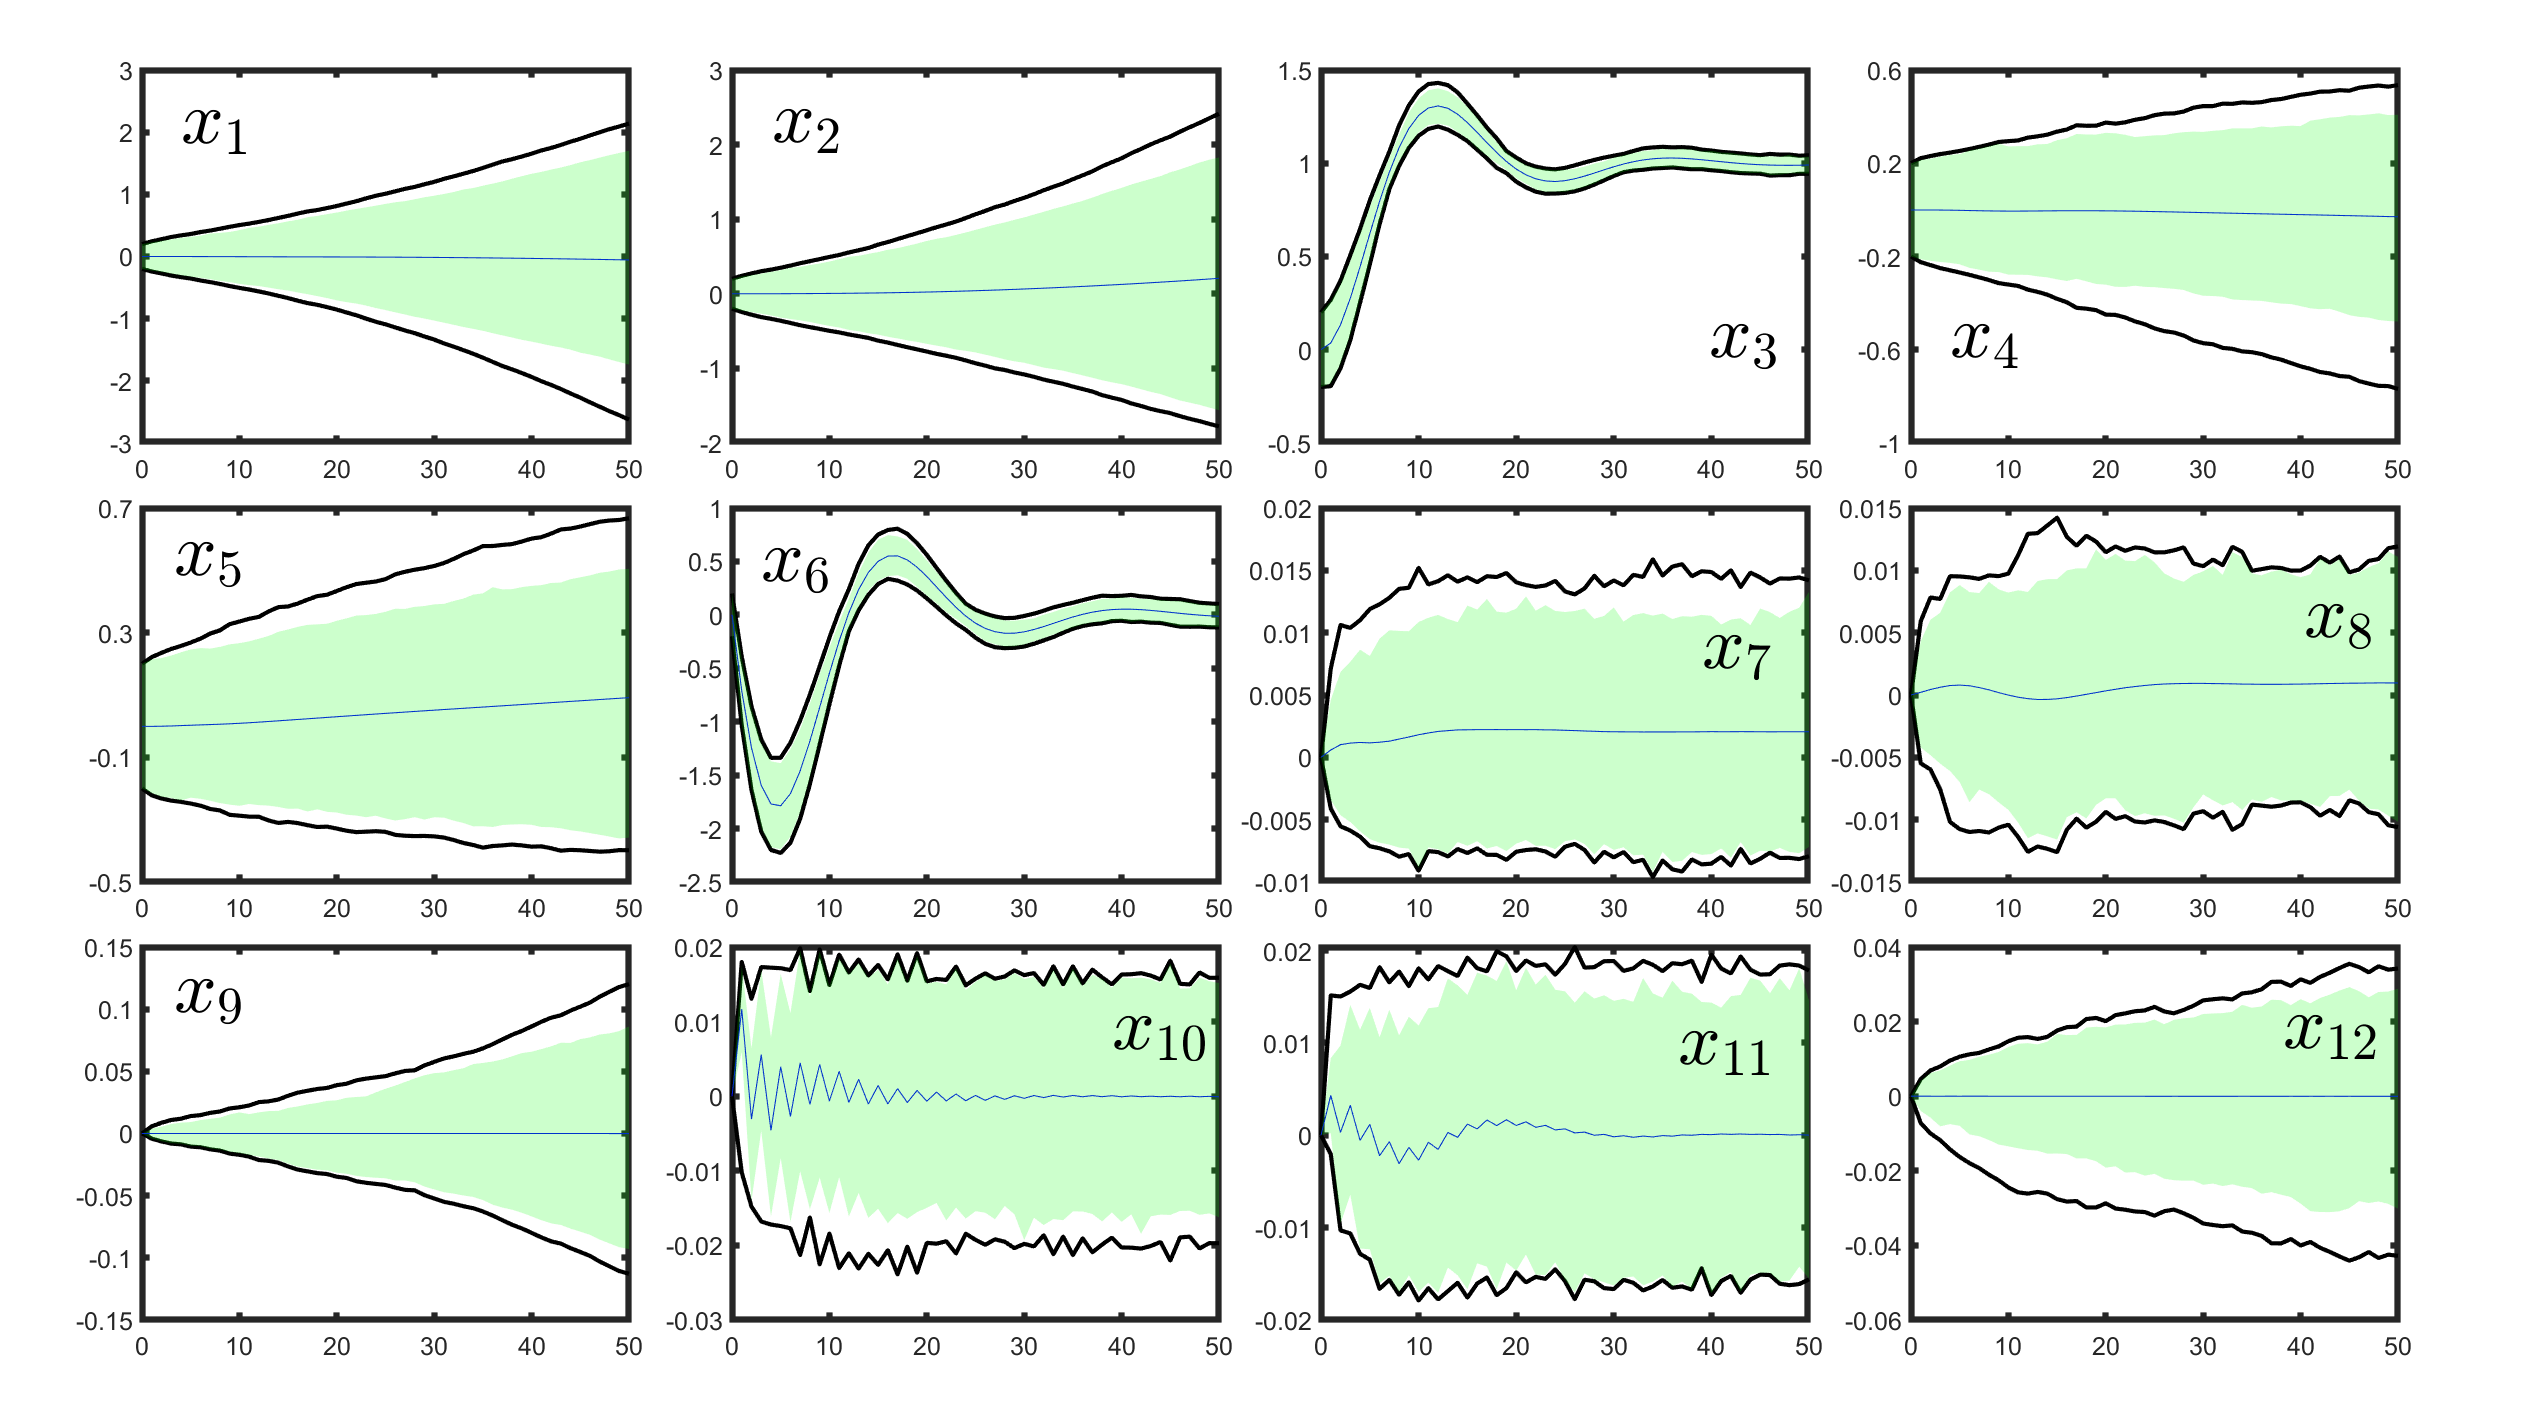
\includegraphics[width = 1.1\textwidth]{figures/final_results_noisyquad.eps}}
    {\caption{Quadcopter: The black lines indicate the probabilistic flowpipe computed using the exact-star technique on the learned surrogate model combined with conformal inference with failure probability $\varepsilon=0.01$. The green shaded areas and blue lines are computed from $100000$ random trajectories from the ODE model. The green area shows the maximum and minimum value of trajectory components over this dataset, and the blue line represents their average value.}
    \label{fig:Quad}}
\end{figure*}




We consider an adaptive cruise controller, a quadcopter, and the Laubloomis benchmarks in \cite{huang2022polar}. In all case studies, we train $1$-step surrogate models that we combine into a $\horizon$-step surrogate model for trajectory prediction. For reachability analysis of the  surrogate model we use the approx-star algorithm from \cite{tran2020nnv} for the Laubloomis case study, while we use the exact-star algorithm from \cite{tran2020nnv} for the adaptive cruise controller and the quadcopter. The underlying system is described by an ordinary differential equation (ODE), potentially affected by noise, and we consider the system at discrete time points. Therefore, we let the control input and the noise be fixed over the sampling time $[\timeid \delta t, (1+\timeid)\delta t], \timeid \in [\horizon]$. The star-sets that we obtain are $n>3$ dimensional. Illustration of our results is thus demonstrated through their projection onto state components. This is important to keep in mind when assessing the tightness of the obtained star-sets.

\myipara{Adaptive Cruise Control}
We consider a $6$-dimensional system consisting of a leader and a follower vehicle that is equipped with an adaptive cruise controller. The underlying black-box model is described by the  ODE model 
\begin{equation}
\label{eq:acc}
\begin{bmatrix}\dot{x}_1\\ \dot{x}_2\\ \dot{x}_3\\ \dot{x}_4\\
\dot{x}_5\\ \dot{x}_6\end{bmatrix} =\begin{bmatrix} x_2\\ x_3\\
-2x_3-4-\mu x_2^2\\ x_5\\ x_6\\ -2x_6+2u-\mu x_4^2\end{bmatrix}+ v, \ \  \init=\left\{  \state_0\ \middle| \  \begin{bmatrix} 90\\32\\0\\10\\30\\0\end{bmatrix} \leq \state_0 \leq \begin{bmatrix} 110\\32.2\\0\\11\\30.2\\0\end{bmatrix} \right\}
\end{equation}
where $v \sim \gaussian(0, d^2)$ with standard deviation $d= \mathbf{diag}([1, 0.1,  0.05,  1,  0.1,  0.05 ])$. The friction coefficient is $\mu=10^{-4}$. The state components $x_1,x_2,x_3$ are the position, velocity, and hidden state of the lead vehicle, while the components $x_4,x_5,x_6$ are the position, velocity, and hidden state of the ego vehicle. The surrogate model is a neural network with ReLU activation functions and with  layers $[6, 32,32,32,6]$. The surrogate model is trained from a training dataset generated from Eq.~\eqref{eq:acc} where the control input $u$ is generated by the adaptive cruise controller. To perform conformal inference, we generate $L=40000$  i.i.d. $50$-step trajectories from Eq.~\eqref{eq:acc} with sampling time $\delta t =0.1 \sec$ that we collect within the test dataset $D_{\text{test}}$. 
% With this number of trajectories,  we can select a minimum failure probability of up to $\varepsilon = \%1$. 
Fig.~\ref{fig:acc_comparison} shows the projections of our probabilistic flowpipe onto its state components by setting $\varepsilon =0.01$. To visualize the tightness of the probabilistic flowpipe, we generate $100000$ additional i.i.d. trajectories from Eq.~\eqref{eq:acc} and include their projection on their state components in Fig.~\ref{fig:acc_comparison} as well. Table \ref{tbl:acc} shows the run time of our experimental results for the range $\varepsilon \in [0.01, 0.1]$.  
% The adaptive cruise controller is a neural network controller that receives the observation, $O=[V_{set},\ t_{gap},\ x_5(\timeid),x_1(\timeid)-x_4(\timeid),\ x_2(\timeid)-x_5(\timeid)]$
% and returns the optimal control to satisfy the proposed STL specification~\eqref{eq:STL-ACC2} within $50$ time steps. Here $V_{set} = 30$, and $t_{gap} = 1.4$ are fixed.
% \begin{equation}\label{eq:STL-ACC2}
% \begin{aligned}
% &\varphi=\alw_{[1,50]} \left[x_1(\timeid)-x_4(\timeid)>d_{safe} \right] 
% \end{aligned}
% \end{equation}
% \begin{table*}[t]
% \centering
% \resizebox{\textwidth}{!}{
% \begin{tabular}{cccccccc} 
% \toprule
% Probability & Calibration & Robustness& Run-time & Probability  & Calibration & Robustness & Run-time  \\
%  Threshold & Dataset size & Range &  &  Threshold & Dataset size & Range \\ 
% \midrule \rowcolor{Gray}
% $0.90$ &  6145  & $\left[ 12.7923,\ 48.2527 \right]$ & 102.0968 $\mathrm{sec}$ &  $0.95$ & 12616  &$\left[ 12.2139,\ 48.2535 \right]$ & 115.4081 $\mathrm{sec}$  \\
% $0.91$ &  6865  &$\left[ 12.7007,\ 48.2530 \right]$ & 103.2027 $\mathrm{sec}$  &  $0.96$ & 15852  &$\left[ 11.8651,\ 48.2532 \right]$ & 126.1511 $\mathrm{sec}$  \\
% \rowcolor{Gray}
% $0.92$ &  7763  &$\left[ 12.6171,\ 48.2529 \right]$ & 104.2707 $\mathrm{sec}$  &  $0.97$ & 21242  &$\left[ 11.1147,\ 48.2537 \right]$ & 151.0995 $\mathrm{sec}$  \\
% $0.93$ &  8919  &$\left[  12.4845,\ 48.2532 \right]$ & 107.4728 $\mathrm{sec}$ &  $0.98$ & 32023  &$\left[ 7.3632,\ 48.2540 \right]$ & 181.9839 $\mathrm{sec}$  \\
% \rowcolor{Gray}
% $0.94$ & 10459  &$\left[ 12.3463,\ 48.2530 \right]$ & 113.9788 $\mathrm{sec}$  &   & & & \\
% \bottomrule
% \end{tabular}
% }
% \caption{Shows the probabilistic guaranteed robustness range for different probability thresholds. Robustness range is computed with Approx-star technique for reachability analysis and conformal inference for risk analysis. In this experiment the calibration dataset size is taken $10\%$ more than the minimum required dataset size for conformal inference. Although the robustness range has provable probabilistic guarantee but the accuracy of bounds is subject to the conservatism in Approx-star technique and the uncertainty caused by the data sampling in conformal inference.} \label{tbl:acc}
% \end{table*} 

% \begin{figure*}[t]
%     \centering
%     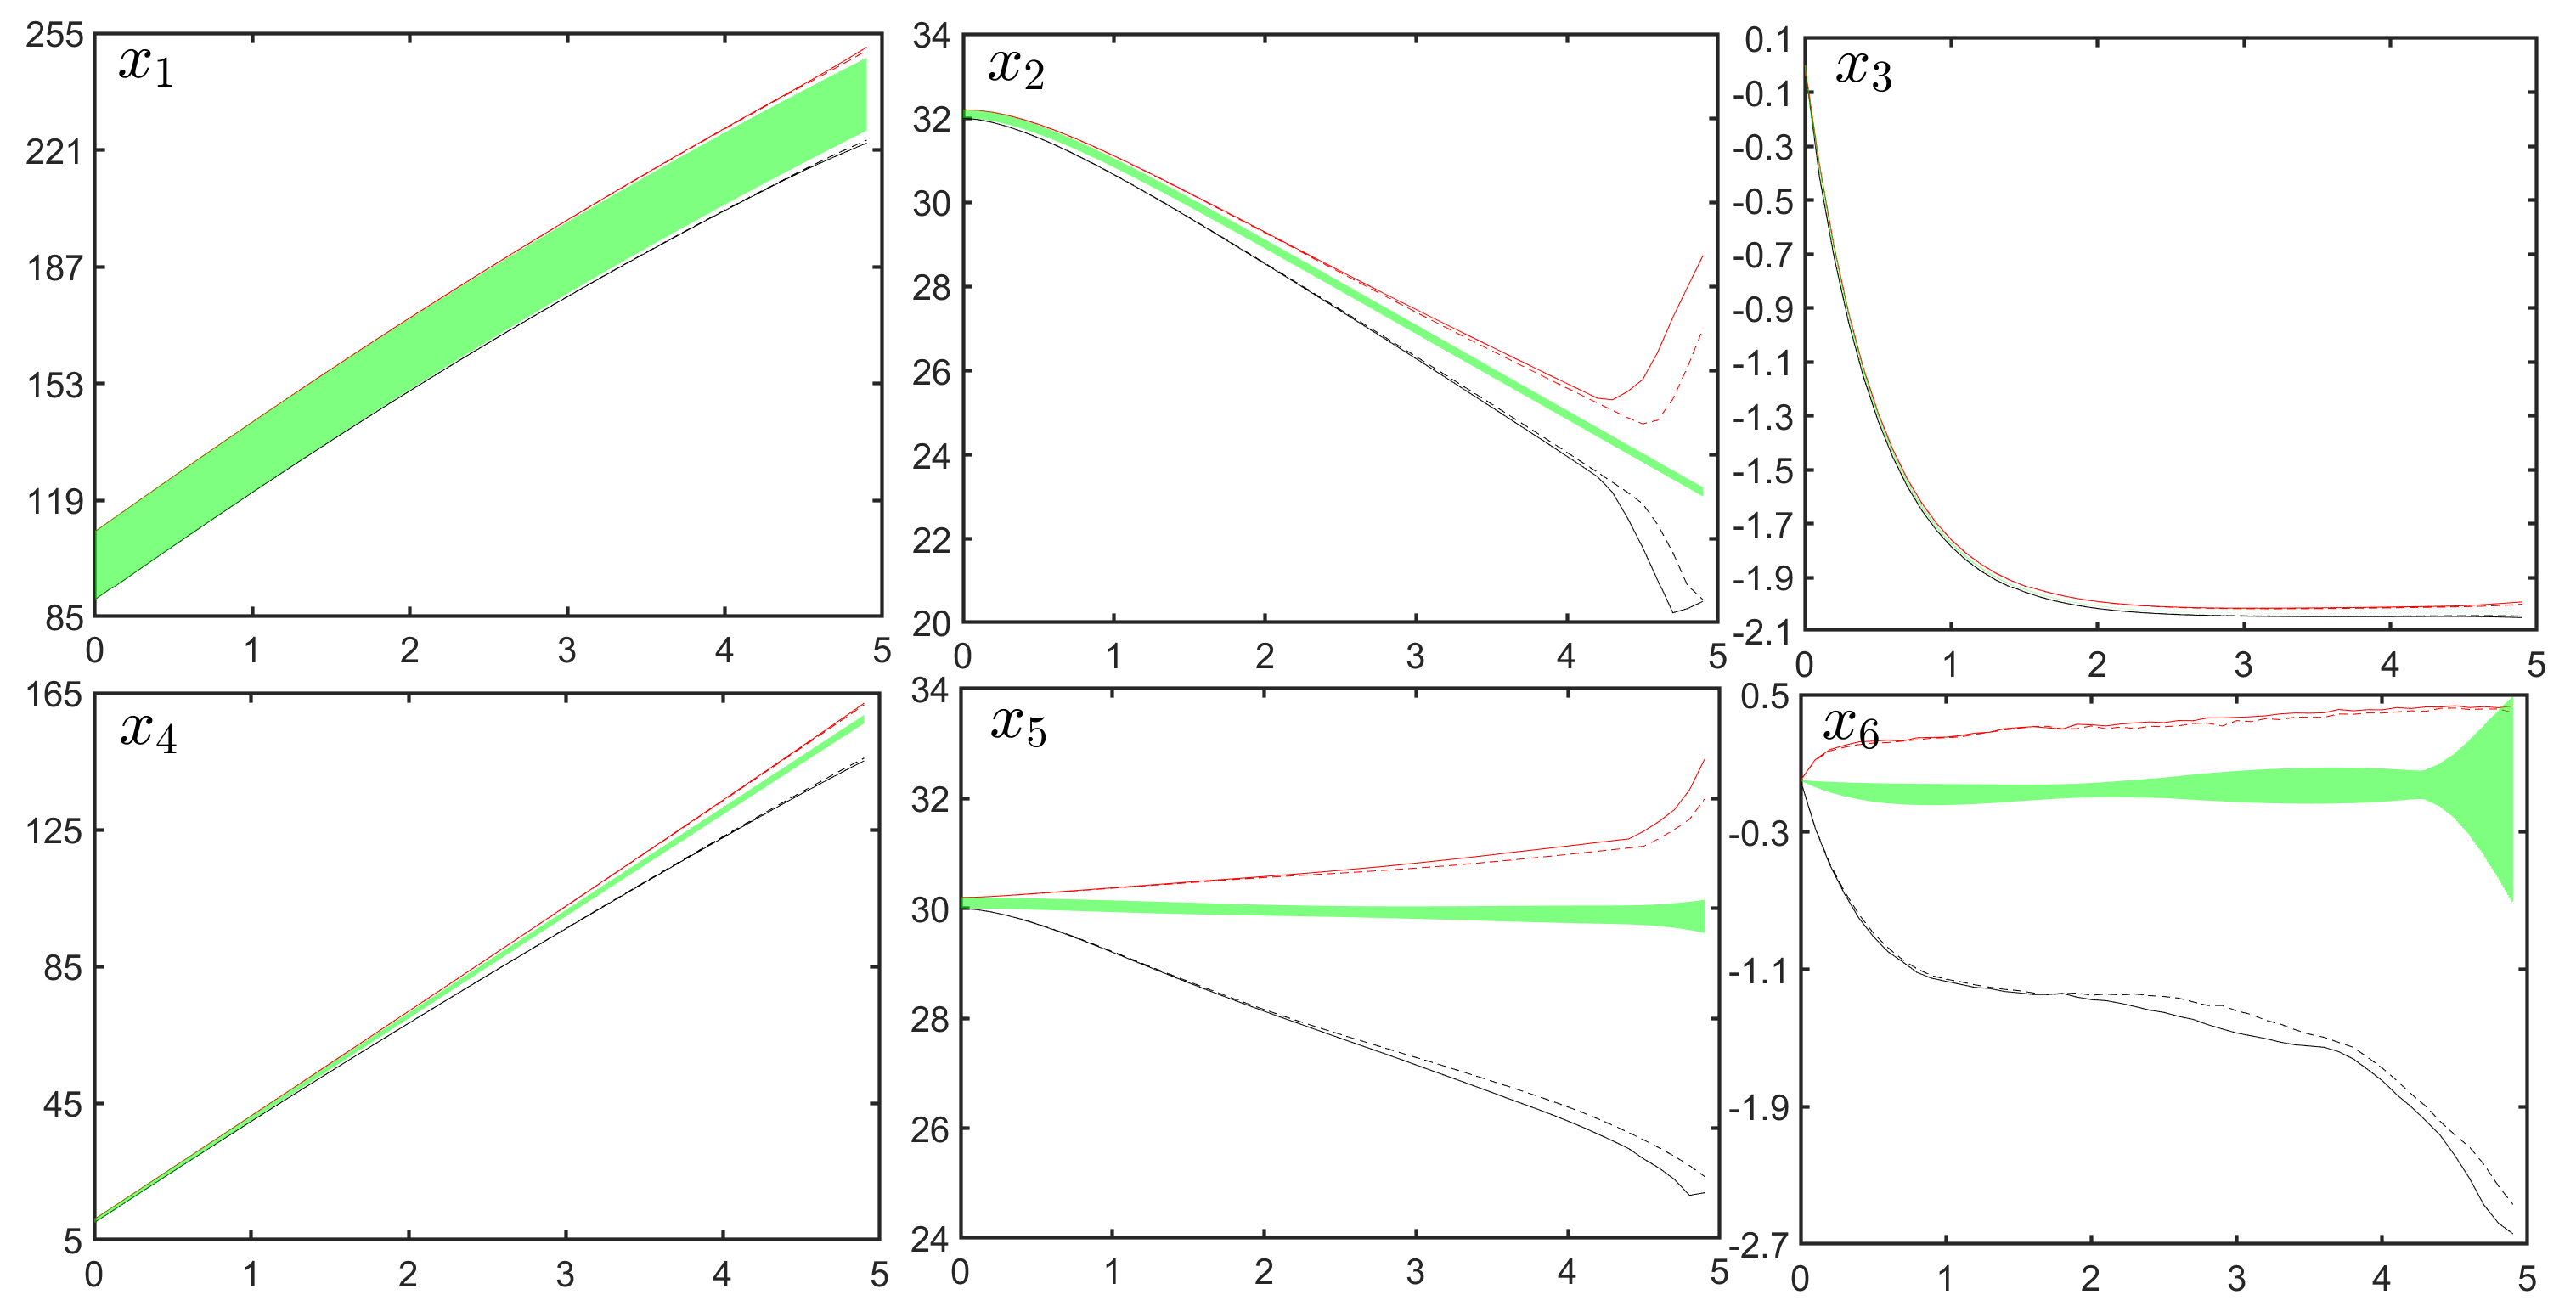
\includegraphics[width = \linewidth]{figures/paper.eps}
%     \caption{Shows the comparison between reachability analysis from single-step dataset and reachability analysis when the black-box model is ideally known. The bounds in dash line shows the reachability analysis with approx-star technique with $\beta=0.95$ and the solid line is for $\beta=0.97$. The green reachset is derived from CORA \cite{} library and represent the exact reach set of black-box model in equation \eqref{eq:acc}, when the model is ideally known.}
%     \label{fig:acc_comparison}
% \end{figure*}


% \begin{table*}[t]
% \centering
% \resizebox{0.9 \textwidth}{!}{
% \begin{tabular}{ccc} 
% \toprule
% Failure & Conformal inference & Reachability  \\
%  Probability & Run-time & Run-time \\ 
% \midrule \rowcolor{Gray}
% $0.10$ &   7.99 $\mathrm{sec}$ & 9.86 $\mathrm{sec}$ \\
% $0.09$ &  8.41 $\mathrm{sec}$ & 9.55 $\mathrm{sec}$  \\
% \rowcolor{Gray}
% $0.08$ &  7.93 $\mathrm{sec}$ & 9.5 $\mathrm{sec}$  \\
% $0.07$ &  7.39 $\mathrm{sec}$ & 9.01 $\mathrm{sec}$ \\
% \rowcolor{Gray}
% $0.06$ & 8.04 $\mathrm{sec}$ & 9.3 $\mathrm{sec}$  \\
% $0.05$ & 7.86 $\mathrm{sec}$ & 9.53 $\mathrm{sec}$  \\
% \rowcolor{Gray}
% $0.04$ & 7.94 $\mathrm{sec}$ & 9.77 $\mathrm{sec}$  \\
% $0.03$ & 8.72 $\mathrm{sec}$ & 9.57 $\mathrm{sec}$  \\
% \rowcolor{Gray}
% $0.02$ & 8.1 $\mathrm{sec}$ & 9.24 $\mathrm{sec}$  \\
% $0.01$ & 9.16 $\mathrm{sec}$ & 7.5 $\mathrm{sec}$  \\
% \bottomrule
% \end{tabular}
% }
% \caption{\small{Shows the computation run-time for probabilistic guaranteed data-driven reachability process for different user-provided failure probabilities. The reachability run time is the overall time for deterministic reachability and inflation of the deterministic reachtube. The reachable sets are computed with exact-star technique for reachability analysis and conformal inference for error analysis. In this experiment. The run-time for training a surrogate $\relu$ model was 2 hours and the run-time for data-generation was 20 minutes.} } \label{tbl:acc}
% \end{table*} 



% \begin{table*}[t]
% \centering
% \resizebox{0.9 \textwidth}{!}{
% \begin{tabular}{cccccc} 
% \toprule
% Failure & Conformal inference & Reachability& Failure  & Conformal inference & Reachability  \\
%  Probability & Run-time & Run-time & Probability & Run-time & Run-time \\ 
% \midrule \rowcolor{Gray}
% $0.10$ &   7.99 $\mathrm{sec}$ & 9.86 $\mathrm{sec}$ &  $0.05$ & 7.86 $\mathrm{sec}$ & 9.53 $\mathrm{sec}$  \\
% $0.09$ &  8.41 $\mathrm{sec}$ & 9.55 $\mathrm{sec}$  &  $0.04$ & 7.94 $\mathrm{sec}$ & 9.77 $\mathrm{sec}$  \\
% \rowcolor{Gray}
% $0.08$ &  7.93 $\mathrm{sec}$ & 9.5 $\mathrm{sec}$  &  $0.03$ & 8.72 $\mathrm{sec}$ & 9.57 $\mathrm{sec}$  \\
% $0.07$ &  7.39 $\mathrm{sec}$ & 9.01 $\mathrm{sec}$ &  $0.02$ & 8.1 $\mathrm{sec}$ & 9.24 $\mathrm{sec}$  \\
% \rowcolor{Gray}
% $0.06$ & 8.04 $\mathrm{sec}$ & 9.3 $\mathrm{sec}$  & $0.01$ & 9.16 $\mathrm{sec}$ & 7.5 $\mathrm{sec}$  \\
% \bottomrule
% \end{tabular}
% }
% \caption{\small{Shows the computation run-time for probabilistic guaranteed data-driven reachability process for different user-provided failure probabilities. The reachability run time is the overall time for deterministic reachability and inflation of the deterministic reachtube. The reachable sets are computed with exact-star technique for reachability analysis and conformal inference for error analysis. In this experiment. The run-time for training a surrogate $\relu$ model was 2 hours and the run-time for data-generation was 20 minutes.} } \label{tbl:acc}
% \end{table*} 





\begin{table*}[t]
\centering
\resizebox{\textwidth}{!}{
\begin{tabular}{ccc||ccc} 
\toprule
Failure & Conformal inference & Reachability& Failure  & Conformal inference & Reachability  \\
 Probability & Run-time & Run-time & Probability & Run-time & Run-time \\ 
\midrule \rowcolor{Gray}
$0.10$ &   2.475 $\mathrm{sec}$ &7.3779 $\mathrm{sec}$ &  $0.05$ & 2.4762 $\mathrm{sec}$ &7.5 $\mathrm{sec}$  \\
$0.09$ & 2.4754 $\mathrm{sec}$ &6.8911  $\mathrm{sec}$  &  $0.04$ & 2.4822 $\mathrm{sec}$ &7.3542 $\mathrm{sec}$  \\
\rowcolor{Gray}
$0.08$ &  2.5894 $\mathrm{sec}$ &7.2825  $\mathrm{sec}$  &  $0.03$ & 2.5316 $\mathrm{sec}$ &7.5548 $\mathrm{sec}$  \\
$0.07$ &  2.6046 $\mathrm{sec}$ &7.5339 $\mathrm{sec}$ &  $0.02$ & 2.364 $\mathrm{sec}$ &7.2504 $\mathrm{sec}$  \\
\rowcolor{Gray}
$0.06$ & 2.4674 $\mathrm{sec}$ &7.1876 $\mathrm{sec}$  & $0.01$ & 3.5858 $\mathrm{sec}$ &7.4376 $\mathrm{sec}$  \\
\bottomrule
\end{tabular}
}
\caption{Quadcopter: Computation times of our method for different user-provided failure probabilities $\varepsilon$. The reachability run-time is the overall time for reachability analysis over the surrogate model and constructing the probabilistic flowpipe with conformal inference. The data generation time for the test dataset is $273\ \sec$ and the run time for training the $\relu$ model on training dataset is  $2$ hours and $25$ minutes. }\label{tbl:Quad}
\end{table*} 



\begin{table*}[t]
\centering
\resizebox{\textwidth}{!}{
\begin{tabular}{ccc||ccc} 
\toprule
Failure & Conformal inference & Reachability& Failure  & Conformal inference & Reachability  \\
 Probability & Run-time & Run-time & Probability & Run-time & Run-time \\ 
\midrule \rowcolor{Gray}
$0.10$ &   89.9305 $\mathrm{sec}$ & 93.8766 $\mathrm{sec}$ &  $0.05$ & 71.3700 $\mathrm{sec}$ & 49.7159 $\mathrm{sec}$  \\
$0.09$ &  72.0818 $\mathrm{sec}$ & 53.0224  $\mathrm{sec}$  &  $0.04$ & 67.8528
$\mathrm{sec}$ & 50.1378 $\mathrm{sec}$  \\
\rowcolor{Gray}
$0.08$ &  74.2623 $\mathrm{sec}$ & 50.0363  $\mathrm{sec}$  &  $0.03$ & 72.8819 $\mathrm{sec}$ & 50.1828 $\mathrm{sec}$  \\
$0.07$ &  71.7105 $\mathrm{sec}$ & 49.7770 $\mathrm{sec}$ &  $0.02$ & 85.9235 $\mathrm{sec}$ & 49.7792 $\mathrm{sec}$  \\
\rowcolor{Gray}
$0.06$ & 69.4149 $\mathrm{sec}$ & 50.7159 $\mathrm{sec}$  & $0.01$ & 91.9276 $\mathrm{sec}$ & 92.9743 $\mathrm{sec}$  \\
\bottomrule
\end{tabular}
}
\caption{Laubloomis: Computation times of our method for different user-provided failure probabilities $\varepsilon$. The reachability run-time is the overall time for reachability analysis over the surrogate model and constructing the probabilistic flowpipe with conformal inference.  The data generation time for the test dataset is $19$ minutes, and the run time for training the $\relu$ model on the training dataset is  $2$ hours and $30$ minutes. }\label{tbl:bench1_laub}
\end{table*} 


% where , $d_{safe}=10+1.4 x_5(\timeid)$. 
 
% \begin{remark}
% Consider the gap between the reachset of black-box and computed bounds, neither necessarily represent the conservatism of approx-star reachability nor conservatism of conformal inference. We generate the bounds using a $50$-step dataset. There exists a variety of different underlying systems that are consistent with this $50$-step dataset. Thus, the failure probability $\varepsilon$ is valid for all of these black-box models, where equation \eqref{eq:acc} represents only a specific example of them. This implies the gap between the green reachable set and the bounds does not necessarily represent the conservatism. For this specific black-box model we observe the state $x_6$ is violating the bounds and our results shows decreasing $\varepsilon$ from $0.1$ to $0.01$ decreases the probability of bound violation.
% \end{remark}
% Here, we analyse the conservatism for verification probability. We first generate $5000$ trajectories from equation \eqref{eq:acc} and check for the portion of trajectories that are entirely inside reachsets $\hat{\states}_\timeid,\ \timeid \in[\horizon]$ and compute the verification probability empirically. We denote this empirical probability with $\beta_{emp}$ and compare it with probability threshold $\beta$. Table \ref{tbl:acc} presents this comparison. 
% \begin{table*}[t]
% \centering
% \resizebox{\textwidth}{!}{
% \begin{tabular}{ccccccccc} 
% \toprule
% Probability & Robustness& Run-time & Probability  & Robustness & Run-time & Probability  & Robustness & Run-time  \\
% Threshold & Range &  & Threshold  & Range & Run-time & Threshold  & Range &   \\ 
% \midrule \rowcolor{Gray}
% $0.90$ & $\left[ 12.7923,\ 48.2527 \right]$ & 102.0968 $\mathrm{sec}$ & $0.93$ & $\left[  12.4845,\ 48.2532 \right]$ & 107.4728 $\mathrm{sec}$ & $0.96$ & $\left[ 11.8651,\ 48.2532 \right]$ & 126.1511 $\mathrm{sec}$ \\
% $0.91$ & $\left[ 12.7007,\ 48.2530 \right]$ & 103.2027 $\mathrm{sec}$ & $0.94$ & $\left[ 12.3463,\ 48.2530 \right]$ & 113.9788 $\mathrm{sec}$ & $0.97$ & $\left[ 11.1147,\ 48.2537 \right]$ & 151.0995 $\mathrm{sec}$ \\
% \rowcolor{Gray}
% $0.92$ & $\left[ 12.6171,\ 48.2529 \right]$ & 104.2707 $\mathrm{sec}$ & $0.95$ & $\left[ 12.2139,\ 48.2535 \right]$ & 115.4081 $\mathrm{sec}$ & $0.98$ & $\left[ 7.3632,\ 48.2540 \right]$ & 181.9839 $\mathrm{sec}$ \\
% \bottomrule
% \end{tabular}
% }
% \caption{Shows the probabilistic guaranteed robustness range for different probability thresholds. Robustness range is computed with Approx-star technique for reachability analysis and conformal inference for risk analysis. Although the robustness range has provable probabilistic guarantee but the accuracy of bounds is subject to the conservatism in Approx-star technique and the uncertainty caused by the data sampling in conformal inference.} \label{tbl:acc}
% \end{table*} 
% \begin{figure*}[t]
% \centering
% \subfloat[Trajectories and bounds in the first dimension]{
% 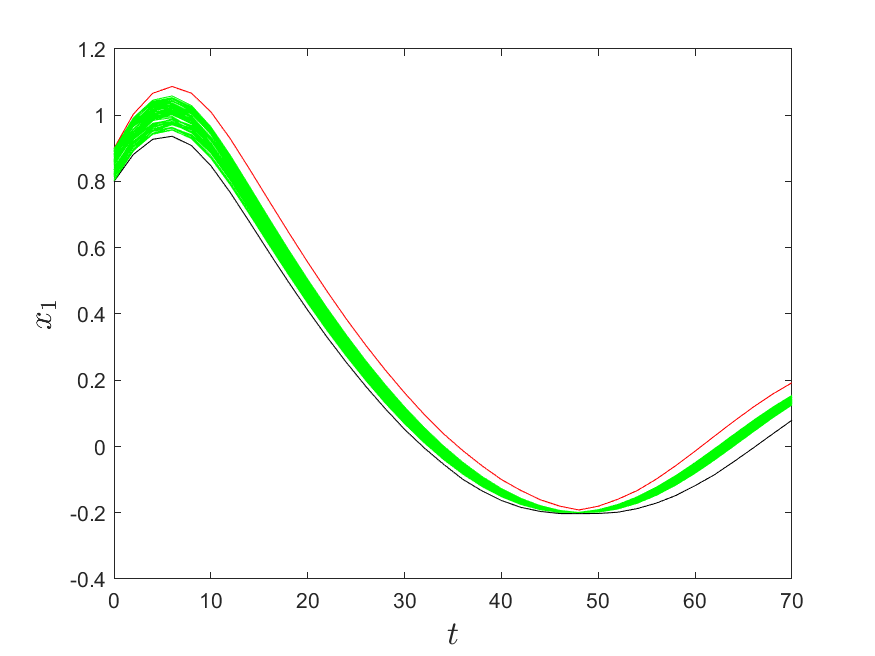
\includegraphics[width=0.35\textwidth]{figures/bound1.png}\label{bench1_1}}
% % \hfill
% \subfloat[Trajectories and bounds in the second dimension.]{%
% 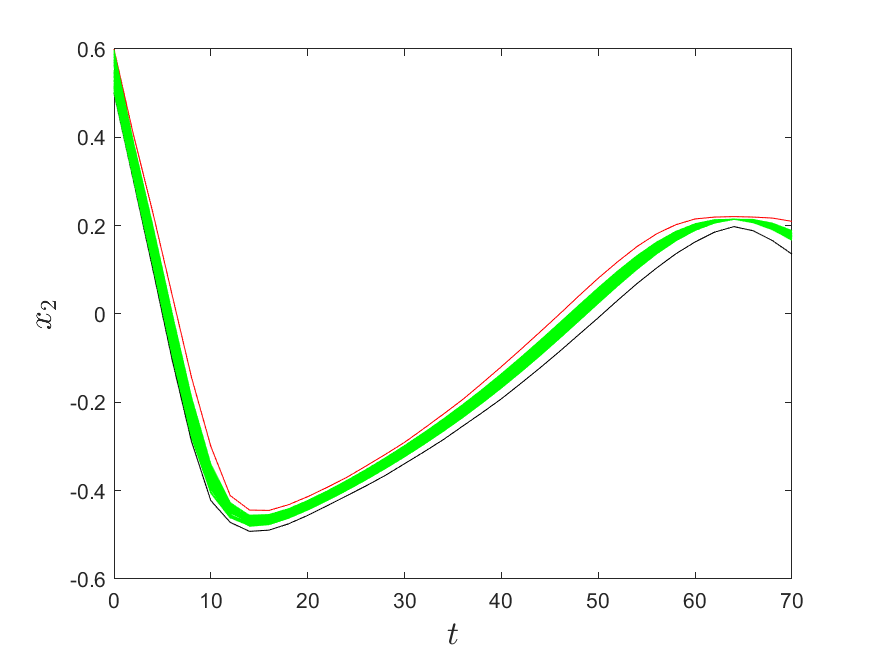
\includegraphics[width=0.35\textwidth]{figures/bound2.png}\label{bench1_2}}%
% % \hfill
% \subfloat[Trajectories and bounds observed from a two-dimensional perspective.]{%
% 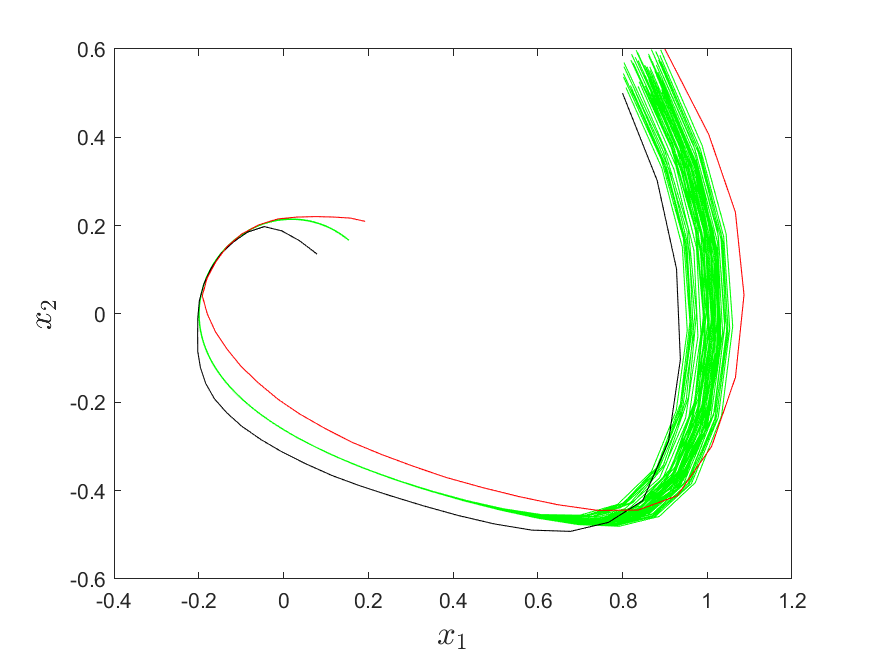
\includegraphics[width=0.35\textwidth]{figures/bound2dim.png}\label{bench1_3}}
%     \caption{The reachability analysis from a one-step dataset. The bounds in the solid line are for $\varepsilon=0.05$. The green trajectories are sampled using the neural network controller in \cite{polar}.Figure \ref{bench1_3} shows a similar result to Figure 3b in \cite{reachnn}.}
%     \label{fig:bench_comparison}
% \end{figure*}



% \begin{figure*}[t]
% \centering
% \subfloat[Trajectories and bounds in the first dimension]{
% 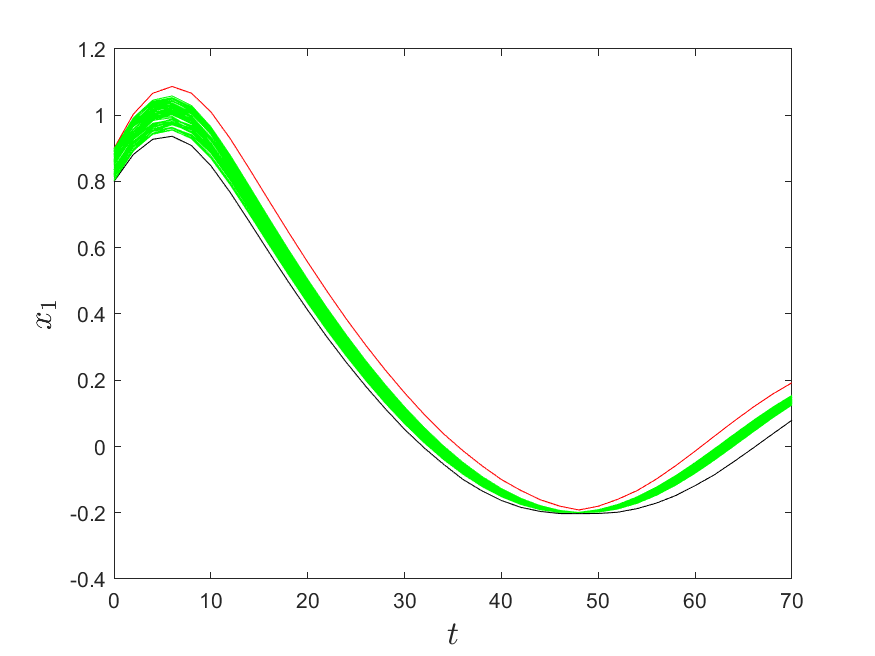
\includegraphics[width=0.48\textwidth]{figures/bound1.png}\label{bench1_1}}
% % \hfill
% \subfloat[Trajectories and bounds in the second dimension.]{%
% 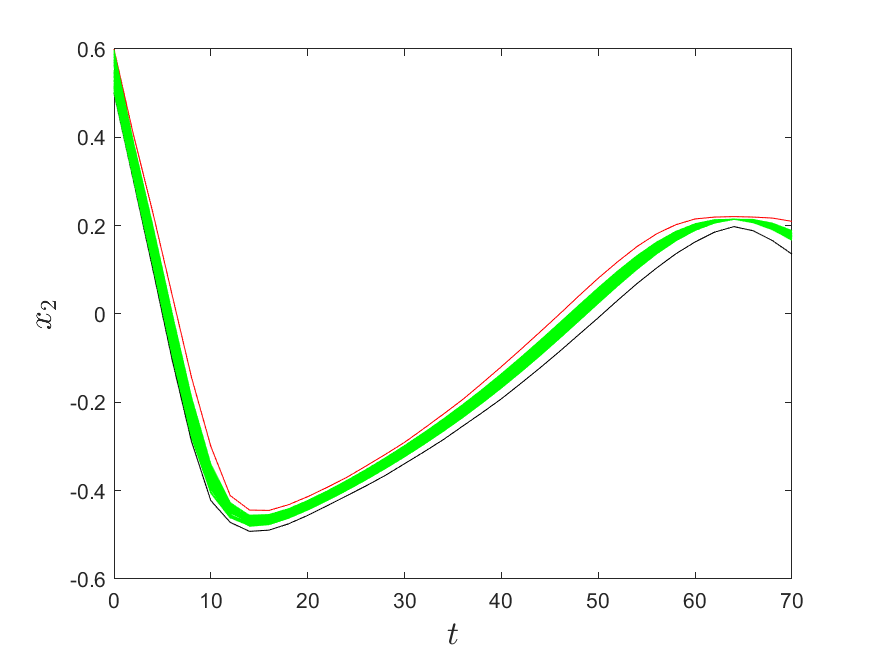
\includegraphics[width=0.48\textwidth]{figures/bound2.png}\label{bench1_2}}%
% % \hfill
%     \caption{The reachability analysis from a $50$-step dataset. The bounds in the solid line are for $\varepsilon=0.05$. The green trajectories are sampled using the neural network controller in \cite{polar}.}
%     \label{fig:bench_comparison}
% \end{figure*}
\myipara{Quadcopter}
We consider a 12-dimensional Quadcopter model that was introduced in \cite{huang2022polar}. The ODE model for the Quadcopter is shown in Eq.~\eqref{eq:Quad12}. The additive noise $v=\left[v_1, v_2, \cdots, v_{12}\right]$ is Gaussian $v \sim \gaussian(0, d^2)$ with standard deviation $d= \mathbf{diag}([0.05\times \vec{1}_{1 \times 6},0.01\times \vec{1}_{1 \times 6}])$. The controller is a neural network controller that was presented in \cite{huang2022polar}. From this model, we generate a test dataset with  $L=40000$ data-points by sampling $50$-step trajectories with sampling time $\delta t = 0.1 \sec$.  We also train our surrogate model as a neural network with  layers $[12,20,20,20,12]$ from an additional training dataset.
\begin{figure*}
{\small 
\begin{equation}\label{eq:Quad12}
    \hspace{-3mm}\left\{ \hspace{-3mm} \begin{array}{ll}
    &\dot{x}_1 = \cos(x_8) \cos(x_9)x_4+( \sin(x_7) \sin(x_8) \cos(x_9)- \cos(x_7) \sin(x_9))x_5\\
    &\hspace{2mm}+( \cos(x_7) \sin(x_8) \cos(x_9)+ \sin(x_7) \sin(x_9))x_6+v_1\\
    &\dot{x}_2 = \cos(x_8) \sin(x_9)x_4+( \sin(x_7)  \sin(x_8)  \sin(x_9)+ \cos(x_7)  \cos(x_9)) x_5\\
    &\hspace{2mm}+( \cos(x_7)  \sin(x_8)  \sin(x_9)- \sin(x_7)  \cos(x_9)) x_6+v_2\\
    &\dot{x}_3 =  \sin(x_8) x_4- \sin(x_7)  \cos(x_8) x_5- \cos(x_7)  \cos(x_8) x_6+v_3\\
    &\dot{x}_4 = x_{12} x_5-x_{11} x_6-9.81  \sin(x_8)+v_4\\
    &\dot{x}_5 = x_{10} x_6-x_{12} x_4+9.81  \cos(x_8)  \sin(x_7)+v_5\\
    &\dot{x}_6 = x_{11} x_4-x_{10} x_5+9.81  \cos(x_8)  \cos(x_7)-9.81-u_1/1.4+v_6\\
    &\dot{x}_7 = x_{10}+( \sin(x_7) ( \sin(x_8)/ \cos(x_8))) x_{11}+( \cos(x_7) ( \sin(x_8)/ \cos(x_8))) x_{12}+v_7\\
    &\dot{x}_8 =  \cos(x_7) x_{11}- \sin(x_7) x_{12}+v_8\\
    &\dot{x}_9 = ( \sin(x_7)/ \cos(x_8)) x_{11}+( \cos(x_7)/ \cos(x_8)) x_{12}+v_9\\
    &\dot{x}_{10} = -0.9259 x_{11} x_{12}+18.5185 u_2+v_{10}\\
    &\dot{x}_{11} = 0.9259 x_{10} x_{12}+18.5185 u_3+v_{11}\\
    &\dot{x}_{12} = v_{12}
    \end{array}
    \right. 
    \begin{array}{l}
    \init= \\
    \left\{  \state_0\ \middle| \  \begin{bmatrix} -0.2\\-0.2\\-0.2\\-0.2\\-0.2\\-0.2\\0\\0\\0\\0\\0\\0\end{bmatrix} \leq \state_0 \leq \begin{bmatrix} 0.2\\0.2\\0.2\\0.2\\0.2\\0.2\\0\\0\\0\\0\\0\\0\end{bmatrix}\right\} 
    \end{array}
\end{equation}}
\end{figure*}
 The run time for our data-driven reachability analysis is shown in Table \ref{tbl:Quad} and the projections of the probabilistic flowpipes onto its state components for $\varepsilon = 0.01$ is shown in Fig.~\ref{fig:Quad}.

\begin{figure*}[t]
\hspace{-7mm}
    {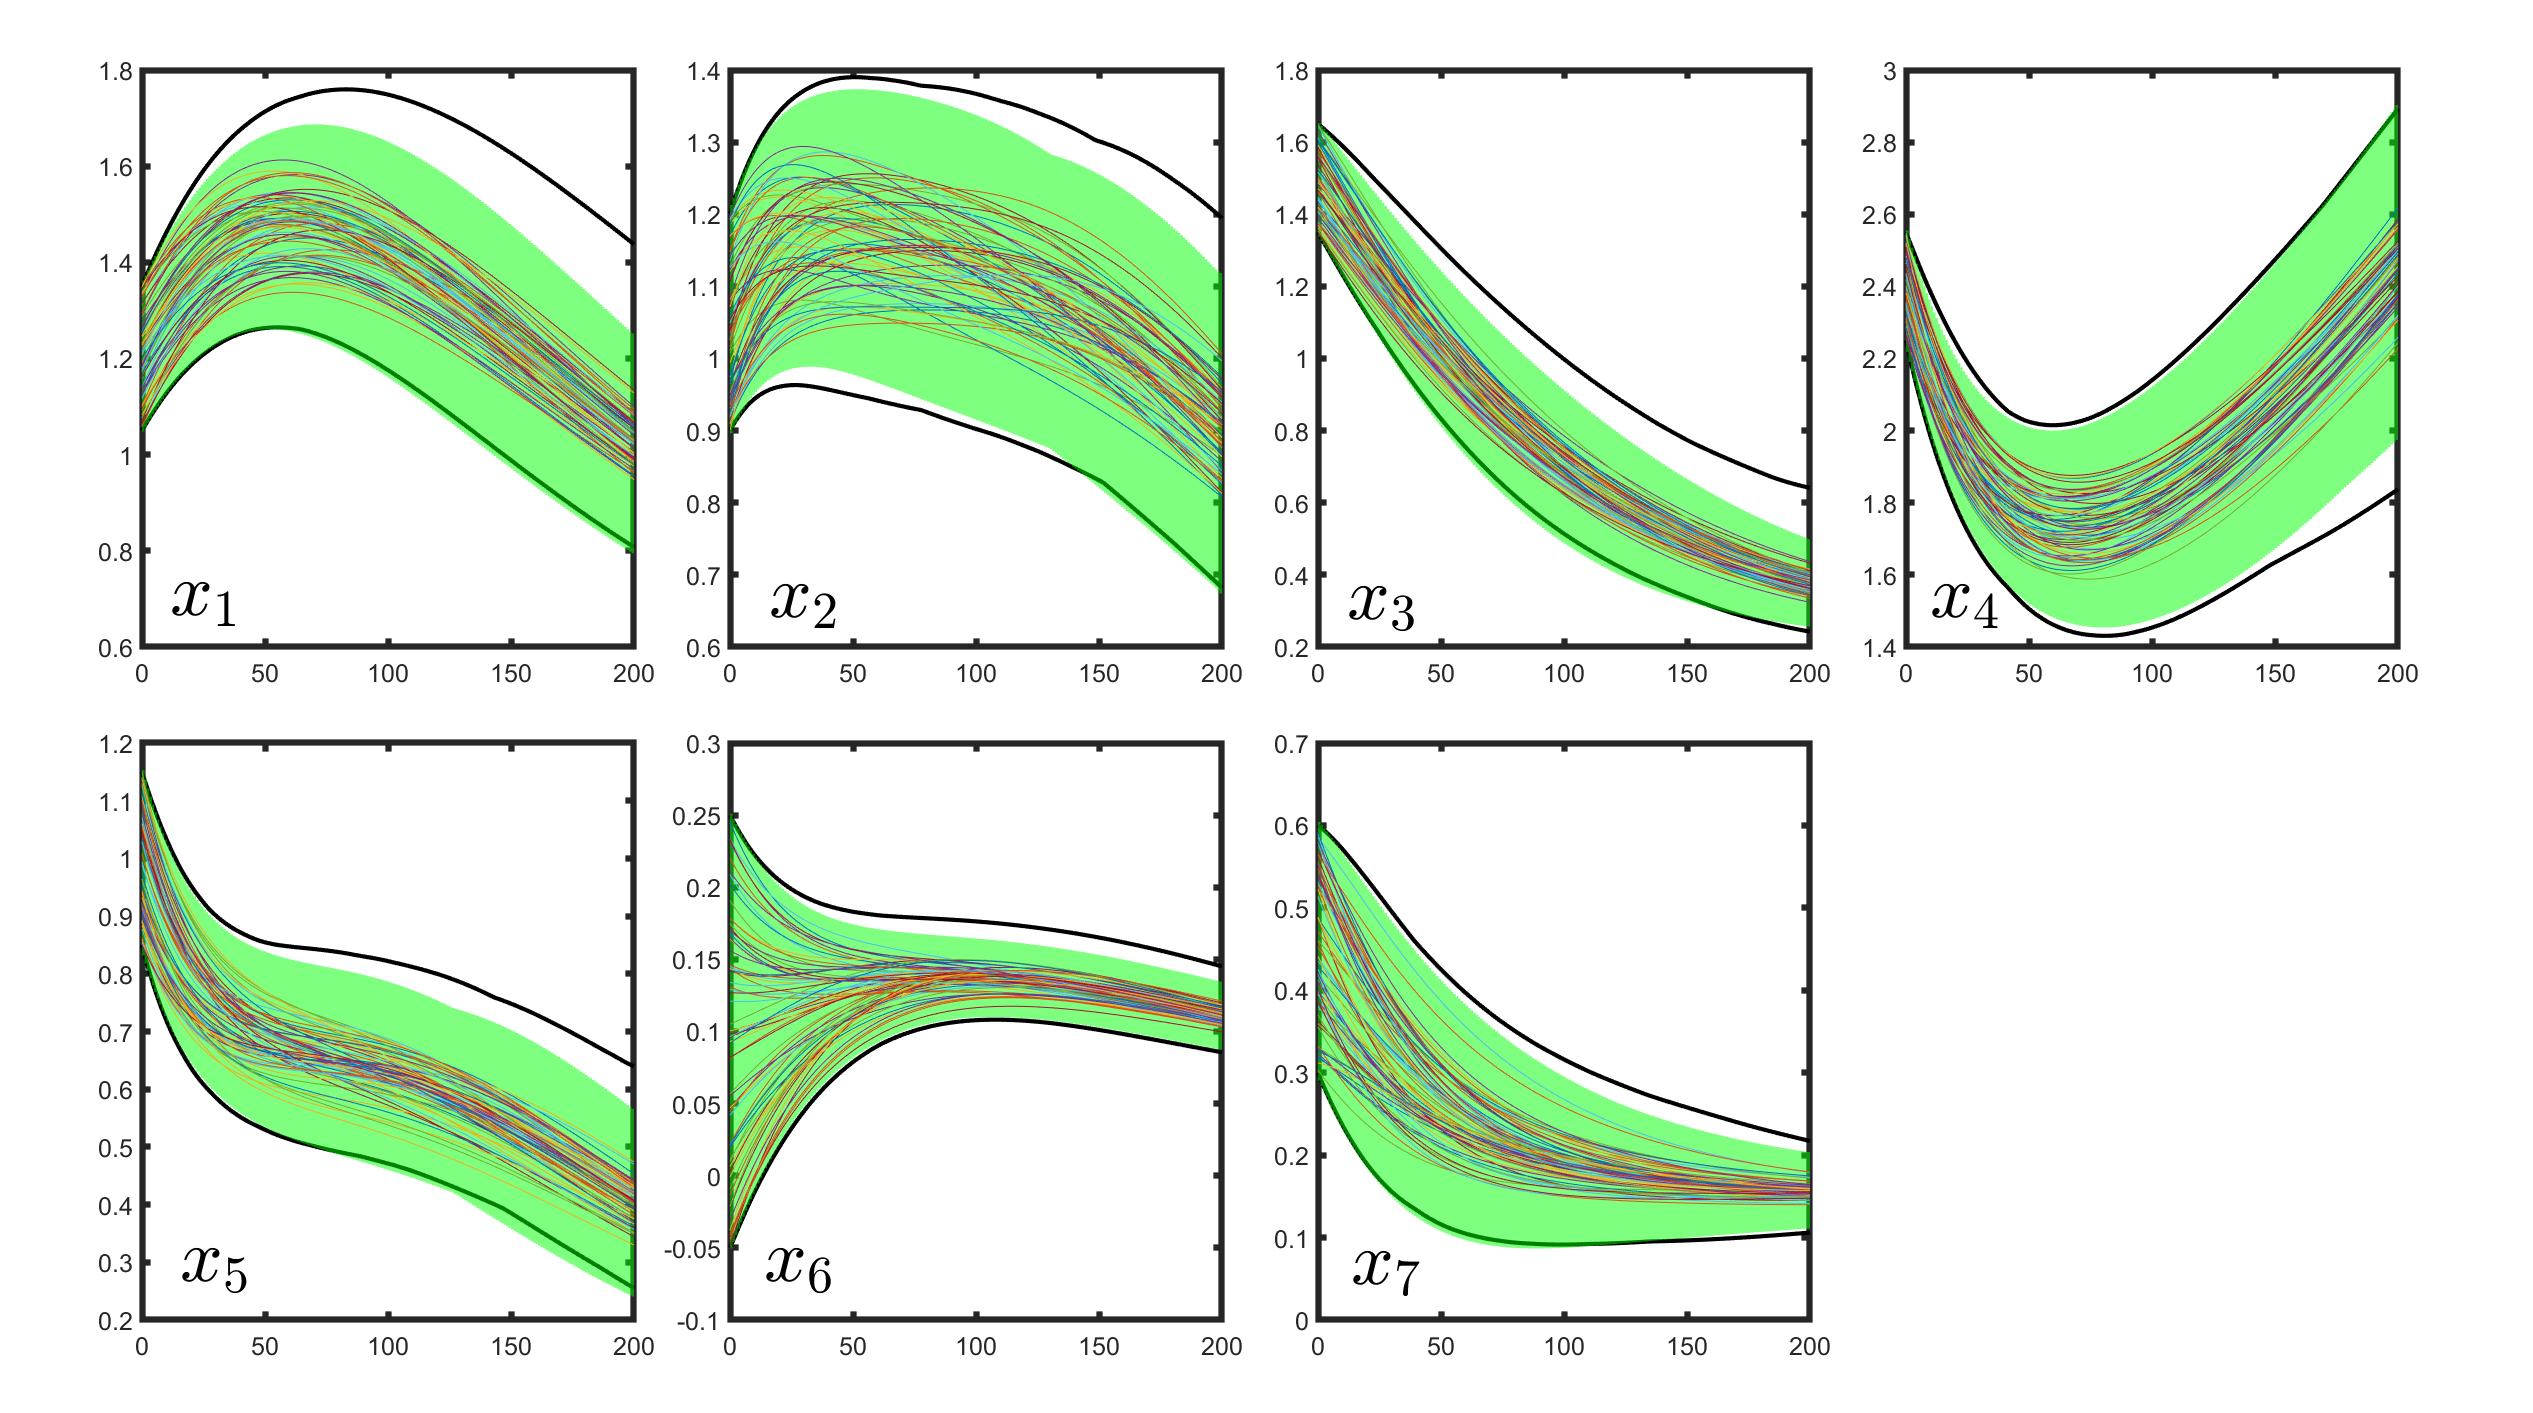
\includegraphics[width=1.1\linewidth]{figures/final_results_laubloomis.eps}}
    {\caption{Laubloomis: Shows our data driven  reachability analysis from $200$-step dataset along with 100 random trajectories generated from $M$. We also included the reachability analysis from CORA toolbox that is based on the ideally known model depicted as green regions. The bounds in black line shows the reachability analysis with approx-star technique combined with conformal inference with prescribed failure probability $\varepsilon=0.01$.}
    \label{fig:laub}}
\end{figure*}
\myipara{Laubloomis}
Finally, we consider a  7-dimensional system which is known as Laubloomis \cite{huang2022polar}. The ODE model  for Laubloomis is shown in Eq.~\eqref{eq:laubloomis}. To provide a comparison with deterministic reachability analysis techniques, we do not add noise to the system in this case so that the system is effectively deterministic. However, note that in our approach we need to sample the initial conditions.  We thus generate a test dataset of size $L =160000$ consisting of $200$-step trajectories with sampling time $\delta t =0.01$. 

\begin{equation}
\label{eq:laubloomis}
\begin{bmatrix}\dot{x}_1\\ \dot{x}_2\\ \dot{x}_3\\ \dot{x}_4\\
\dot{x}_5\\ \dot{x}_6\\ \dot{x}_7\end{bmatrix} =\begin{bmatrix} 1.4 x_3-0.9 x_1\\ 2.5 x_5-1.5 x_2\\
0.6  x_7-0.8 x_3 x_2\\ 2.0-1.3 x_4 x_3\\ 0.7 x_1-1.0 x_4 x_5\\ 0.3 x_1-3.1 x_6 \\ 1.8 x_6-1.5  x_7 x_2
 \end{bmatrix}, \ \  \init=\left\{  \state_0\ \middle| \  \begin{bmatrix} 1.05\\ 0.9\\ 1.35\\ 2.25\\ 0.85\\ -0.05\\ 0.3 \end{bmatrix} \leq \state_0 \leq \begin{bmatrix} 1.35\\ 1.2\\ 1.65\\ 2.55\\ 1.15\\ 0.25\\ 0.6\end{bmatrix} \right\}
\end{equation}

Again, we train a surrogate model as a neural network with $\relu$ activation functions and layers $[7,20,20,20,7]$.  Since the horizon length of trajectories is long, we utilize the approx-star approach instead of the exact-star approach which is more efficient at the cost of conservatism. The simulation of the results for $\varepsilon = 0.01$ is also demonstrated in Fig.\ref{fig:laub}. The reachability run time for our data driven probabilistic approach for a range of failure probabilities $\varepsilon \in [0.01, 0.1 ]$ is shown in Table \ref{tbl:bench1_laub}. Finally, we  utilize the CORA toolbox \cite{althoff2015introduction} to compare to our results, which is shown in Fig.\ref{fig:laub}. We emphasize that  the CORA toolbox is only applicable to deterministic systems and assumes access to the model, while our approach only assumes availability of data.



% \myipara{Benchmark one}
% We consider a benchmark 2-dimensional system introduced in \cite{polar}. We generate a test datasets to evaluate our approach by sampling $35$-step trajectories. Each test dataset comprises 40000 samples. The ODE function used in the benchmark is presented below:
% \begin{equation}
%     \label{eq:bench1}
% \resizebox{\hsize}{!}{$
% \begin{bmatrix}\dot{x}_1\\ \dot{x}_2
% \end{bmatrix} =\begin{bmatrix} x_2\\ ux_2^2 - x_1\\
% \end{bmatrix}, \ \  \init=\left\{  \state_0\ \middle| \  \begin{bmatrix} 0.8\\0.5\end{bmatrix} \leq \state_0 \leq \begin{bmatrix} 0.9\\0.6\end{bmatrix} \right\}$}
% \end{equation}
% We acquire the control input, denoted as $u$, from a neural network controller that takes in the observation $O=[x_1(\timeid), x_2(\timeid)]$ and is designed to achieve the goal set within 35 time steps. The neural network controller used in our approach is the same as the one used in the benchmark, with the goal set for the controllers defined as $x_1 \in [0, 0.2]$ and $x_2 \in [0.05, 0.3]$. The run time is shown in table \ref{tbl:bench1}.









